\documentclass[12pt, titlepage]{article}
\usepackage[section]{placeins}
\usepackage{booktabs}
\usepackage{tabularx}
\usepackage{graphicx}
\graphicspath{ {./} }
\usepackage{amssymb}
\usepackage{threeparttable}
\usepackage{hyperref}
\usepackage{placeins}
\usepackage{natbib}
\bibliographystyle{plain}
\usepackage[nottoc]{tocbibind}

\hypersetup{
    colorlinks,
    citecolor=black,
    filecolor=black,
    linkcolor=red,
    urlcolor=blue
}

\title{SE 3XA3: User Guide\\CraftMaster}

\author{Group 307, 3 Craftsmen\\
		Hongqing Cao 400053625\\
		Sida Wang	 400072157\\
		Weidong Yang 400065354}



\date{\today}


\begin{document}

\maketitle

\pagenumbering{roman}
\tableofcontents
\listoftables
\listoffigures
\FloatBarrier
\begin{table}
\begin{tabularx}{\textwidth}{p{3cm}p{2cm}X}
\toprule {\bf Date} & {\bf Version} & {\bf Notes}\\
\midrule
Feb 29th & 1.0 & General Content upload\\
Mar 26th & 2.0 & Final Update for Rev1\\
\bottomrule
\end{tabularx}
\caption{\bf Revision History}
\end{table}
\FloatBarrier
\clearpage

\pagenumbering{arabic}

\section{Overview}
This document acts as a guide book for players who want to learn to play the game.
\section{Terminologies}
\begin{table}[htbp]
\begin{tabularx}{\textwidth}{p{2cm}X}
\toprule {\bf Term} & {\bf Definition}\\
\midrule
OS & Computer Operating System\\
PC & Personal Computer\\
\bottomrule
\end{tabularx}
\caption{\bf Terminologies}
\end{table}
\section{How to install the game on your PC?}
The game is supported on both Windows OS and Linux OS. Both versions can be simply downloaded as zip files from the download page of the  \href{http://rexwangsida.pythonanywhere.com/}{GAME WEBSITE}. Once the zip file is downloaded and decompressed, it is ready to be started and played.
\section{How to start the game?}
The game is supported in executable file format. To start the game, you can go into the decompressed zip file and find the file named "CraftMaster" with the game logo as its icon, which is shown in figure 1 below. Placing the cursor on the icon of the file and a double left-clicks will automatically start the game.
 
\FloatBarrier

\begin{figure}[h]
\centering
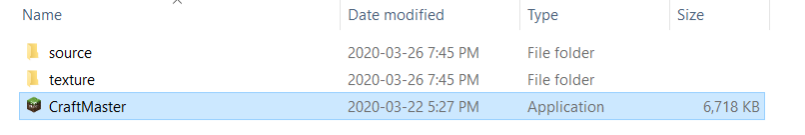
\includegraphics[scale=0.7]{file}
\caption{Game File}
\end{figure}
\FloatBarrier

\section{How to play?}

\subsection{Start the Game}
The Main Menu, Game Menu, and Loading Menu are shown in the figures below in figure 2, figure 3, and figure 4. To start the game, clicking on the "start Game" button and select a game loading mode. The game loading can be divided into "Start New Game" and "Load Game". With the "Load Game" option, the player can play in a game world that was previously saved. If the player selects the "Load Game" option, there are two game savings(Game one and Game two) to be selected, which are based on previous game savings.
\FloatBarrier

\begin{figure}[h]
\centering
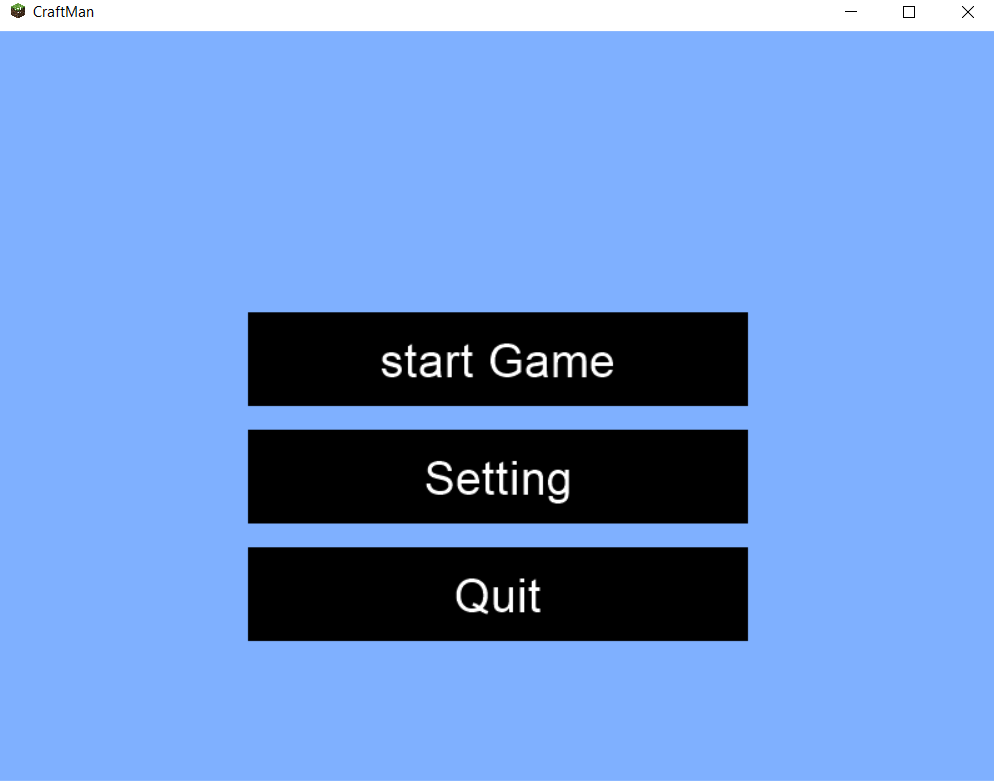
\includegraphics[scale=0.25]{mainmenu}
\caption{Main Menu}
\end{figure}
\FloatBarrier
\begin{figure}[h]
\centering
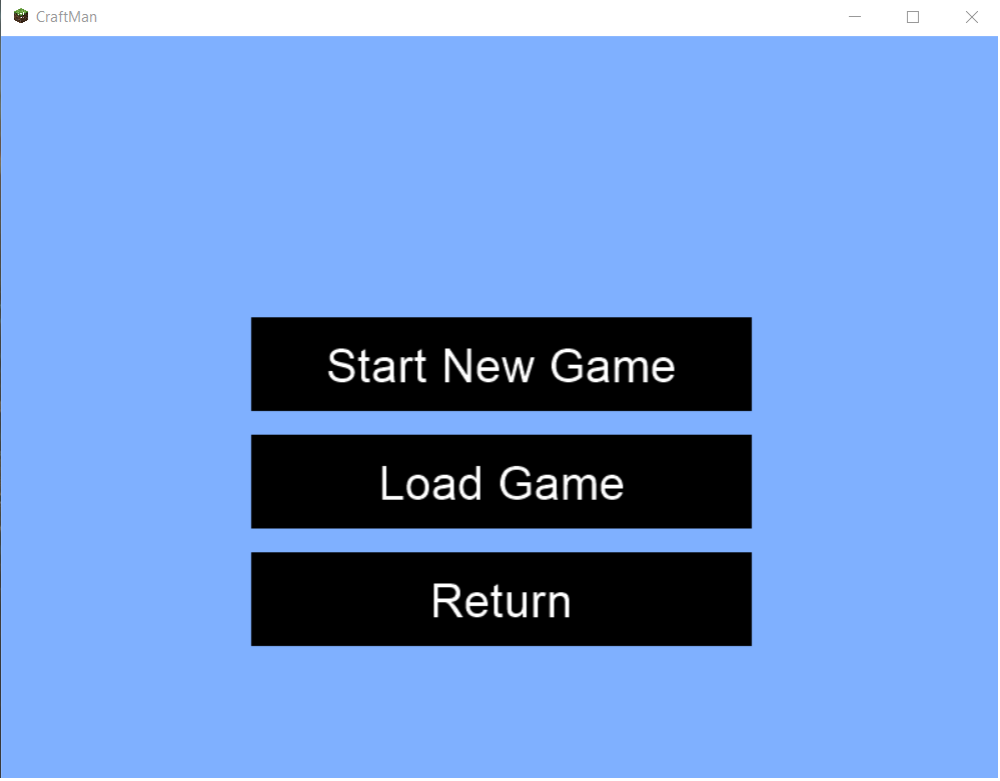
\includegraphics[scale=0.25]{gamemenu}
\caption{Game Menu}
\end{figure}
\FloatBarrier
\FloatBarrier
\begin{figure}[h]
\centering
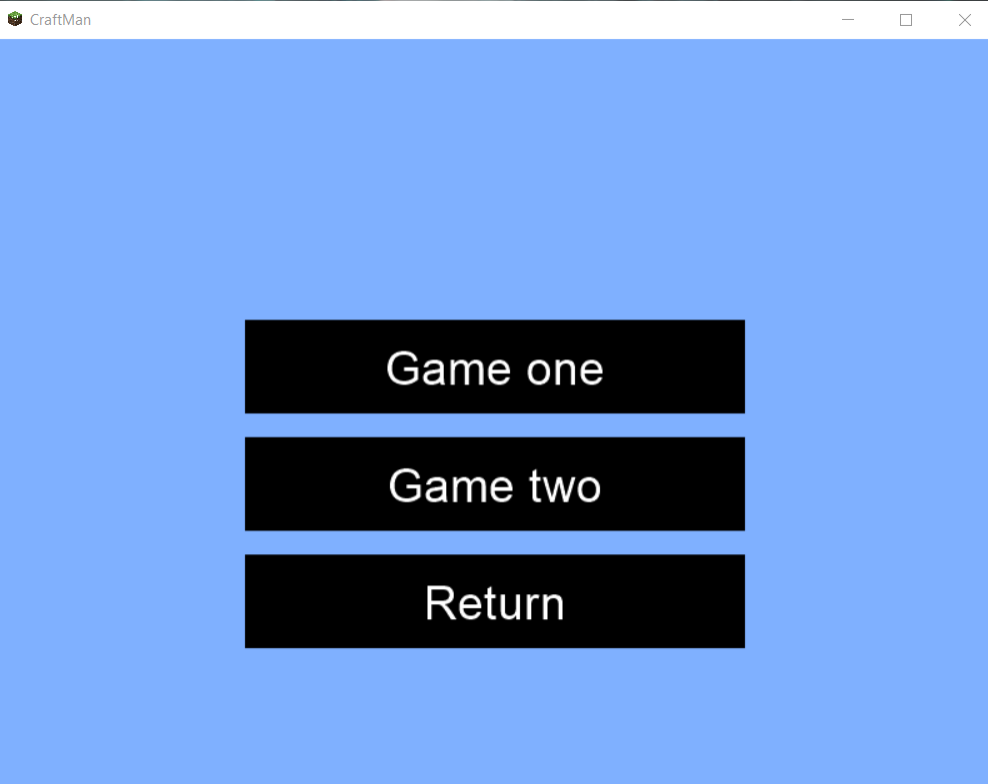
\includegraphics[scale=0.25]{loadingmenu}
\caption{Loading Menu}
\end{figure}
\FloatBarrier

\subsection{In-Game Operations}
\subsubsection{Mouse-based Operations}
\begin{table}[!htbp]
\centering
\begin{tabular}{ |c|c| }
\hline
 \textbf{Mouse Input} & \textbf{Operation(s)} \\ \hline
 Movement & Change the direction of the character \\ \hline
 Left-click & Destroy a block \\ \hline
 Right-click & Build a block \\ \hline
\end{tabular}
\caption{\textbf{Mouse-based Operations}}
\end{table}
\FloatBarrier


\subsubsection{Keyboard-based Operations}
\begin{table}[!htbp]
\centering
\begin{tabular}{ |c|c| }
\hline
 \textbf{Keyboard Input} & \textbf{Operation(s)} \\ \hline
 W & Move Forward \\ \hline
 A & Move to the left \\ \hline
 S & Move backward \\ \hline
 D & Move to the right \\ \hline
 Space & Jump \\ \hline
 Tab & Toggle flying mode\\ \hline
 ESC & Release Cursor from the game window and show ESC menu\\ \hline
 1 & Switch the block building type to brick\\ \hline
 2 & Switch the block building type to grass\\ \hline
 3 & Switch the block building type to stone\\ \hline
\end{tabular}
\caption{\textbf{Keyboard-based Operations}}
\end{table}


\subsection{Change the Day-Night Mode}
The Day-Night Mode can be changed on the Setting Menu before the game starts or on the ESC menu when the game is running.
\subsubsection{Change it on the Setting Menu}
To change it on the Setting Menu, clicking on the "Setting" button on the Main Menu(shown in figure 2) and then clicking on the day-night switch(shown below in figure 5).
\FloatBarrier
\begin{figure}[h]
\centering
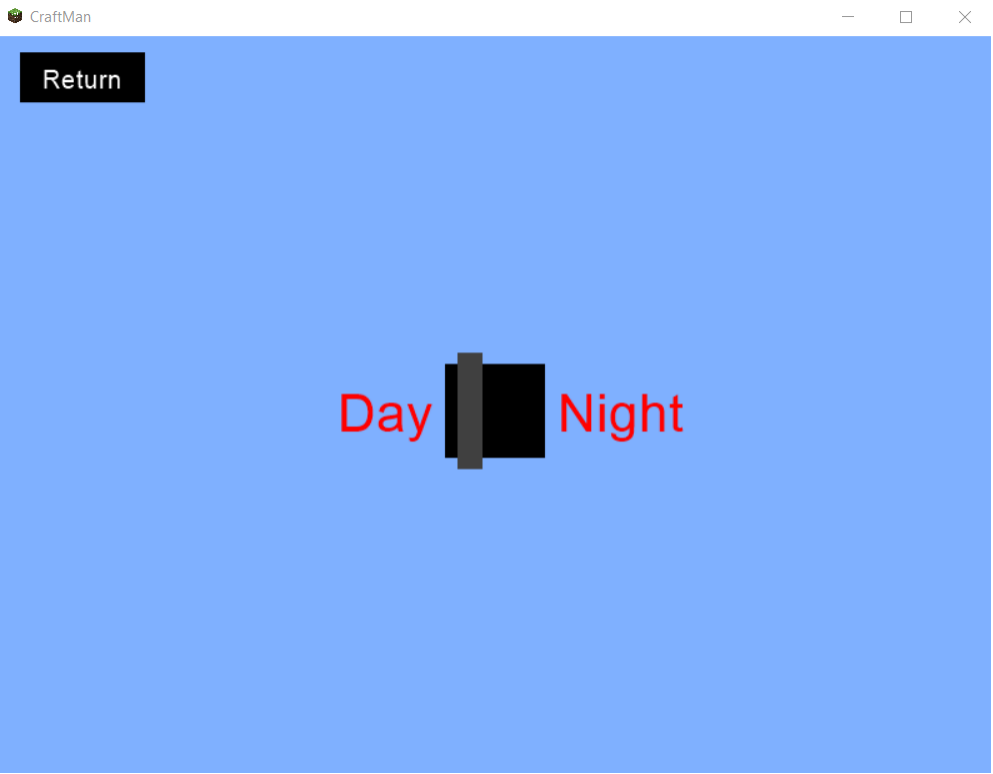
\includegraphics[scale=0.25]{settingmenu}
\caption{Setting Menu}
\end{figure}
\FloatBarrier
\subsubsection{Change it on the ESC Menu}
To change it on the ESC Menu, clicking the ESC key on the keyboard while in game and then clicking on the day-night switch(shown below in figure 6).
\FloatBarrier
\begin{figure}[h]
\centering
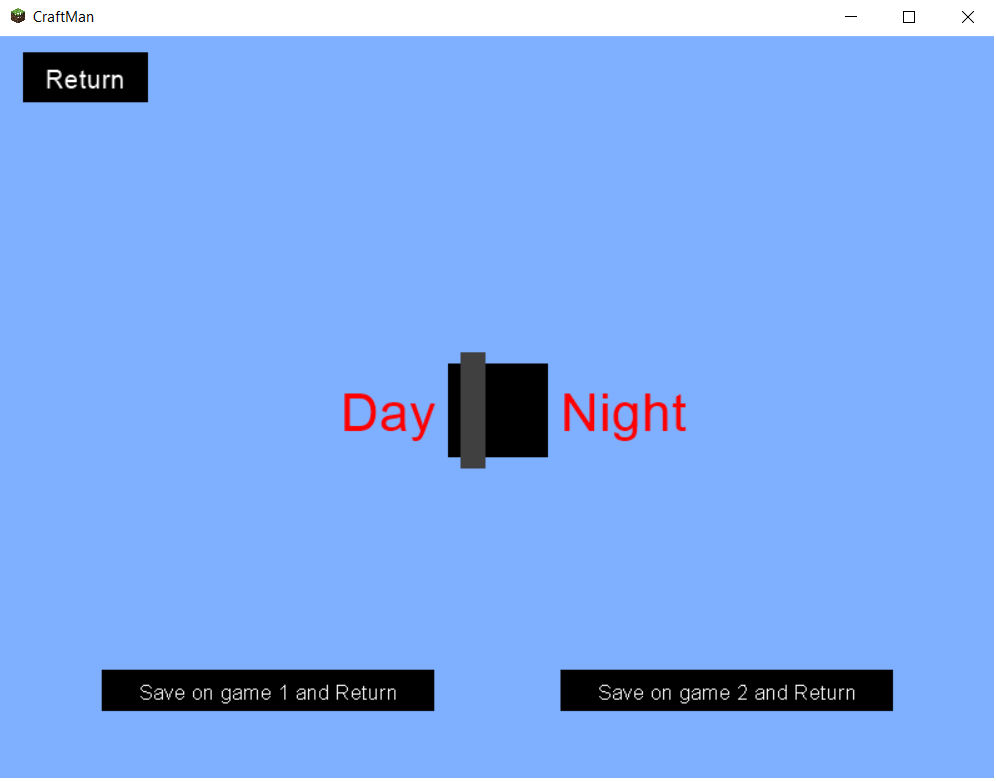
\includegraphics[scale=0.25]{ESCmenu}
\caption{ESC Menu}
\end{figure}
\FloatBarrier



\subsection{Save and Exit the Game}
Once you release the cursor by clicking on "ESC" on the keyboard and the ESC Menu shows, choose an option to save to "game 1" or "game 2" by clicking on the saving buttons on the ESC Menu(shown in figure 6). This will automatically save the game scene and direct you to the Game Menu(shown in figure 3). To quit the game, clicking on the “Return” button on the Game Menu and then clicking on the "Quit" button on the Main Menu.

\section{Something to be aware of}
Any folder or file in the game folder beside the game file itself must not be changed or modified, or the game might not function well.
\end{document}